%% ------------------------------------------------------------------------- %%
\chapter{Introdução}
\label{cap:introducao}

Test-Driven Development (TDD) é uma das práticas mais populares da Programação
Extrema (XP) \cite{XPExplained}. 
Na opinião de muitos autores conhecidos, TDD agrega diversos benefícios ao
código produzido, dentre eles, simplicidade, foco, melhor design, entre outras.

Por esses motivos, é possível observar a crescente adoção e procura por TDD
através do número de pesquisas publicadas pela academia (muitas delas citadas no
capítulo \ref{cap:trabalhos-relacionados}). Em 2010, foi realizado o Primeiro
Workshop Internacional de Test-Driven Development, na cidade de Paris, 
organizado pela Dra. Laurie Williams \footnote{http://agile.csc.ncsu.edu/tdd/. 
Último acesso em 29/outubro/2010}.

Em um questionário de 2010, organizado por Scott Wambler, chamado de \textit{How
Agile Are You?} \cite{wambler-survey-agile}, mostra que 53\% dos times ágeis
adotaram TDD como uma maneira para validar o trabalho feito, conforme mostra a 
figura \ref{wambler-agile-2010}. Outro questionário de 2008, 
chamado de \textit{Test Driven Development (TDD) Survey}
\cite{wambler-survey-tdd}  mostra que 57\% dos desenvolvedores utilizam TDD como
técnica para capturar informações de design, conforme mostrado na figura 
\ref{wambler-tdd-2008}. 

No Brasil, é possível observar o crescente número de pessoas atrás de
informações sobre a prática nas mais diversas listas de discussão e fóruns sobre
tecnologia, como o GUJ \footnote{\url{http://www.guj.com.br}.
Último acesso em 27 de fevereiro 2011} ou o .NET Architects 
\footnote{\url{http://www.dotnetarchitects.net/}. Last access on February
27 de fevereiro de 2011}. Diversos eventos de desenvolvimento de
software realizados no Brasil em 2010, como a QCON SP
\footnote{\url{http://www.qconsp.com/}. Último acesso em 02 de março de 2011} e
a Agile Brazil \footnote{\url{http://http://www.agilebrazil.com/}. Último acesso
em 02 de março de 2011} também contaram com palestras sobre o assunto.

Além disso, programadores que experimentam a prática e percebem seus
efeitos, raramente voltam atrás. Os aficionados por TDD dizem que estão
\textit{``infectados pelo teste''} \cite{tdd-fearless}.

Apesar de todos os possíveis vieses das informações apresentadas acima, os
números mostram que uma grande parte dos desenvolvedores ágeis já utilizam a 
prática no seu dia-a-dia.

% TODO: centralizar duas figuras
\begin{figure}
	\centering
	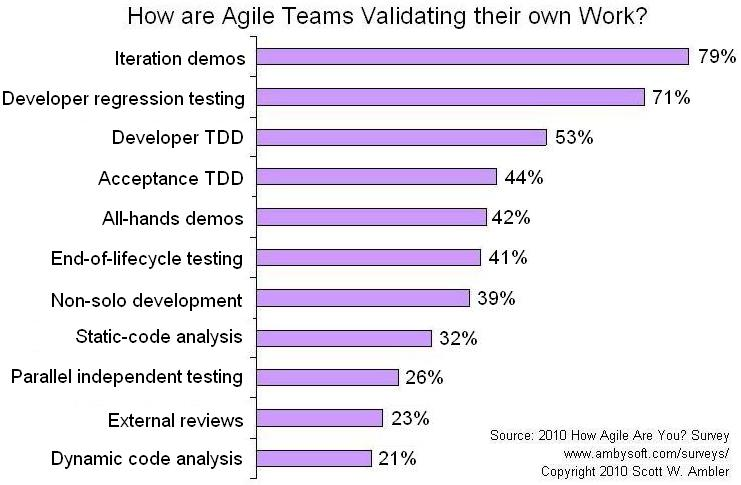
\includegraphics[scale=.4]{agileCriteria2010Validating}
	\caption{Como times ágeis validam seu próprio trabalho?}
	\label{fig:wambler-agile-2010}
\end{figure}
	
\begin{figure}
	\centering
	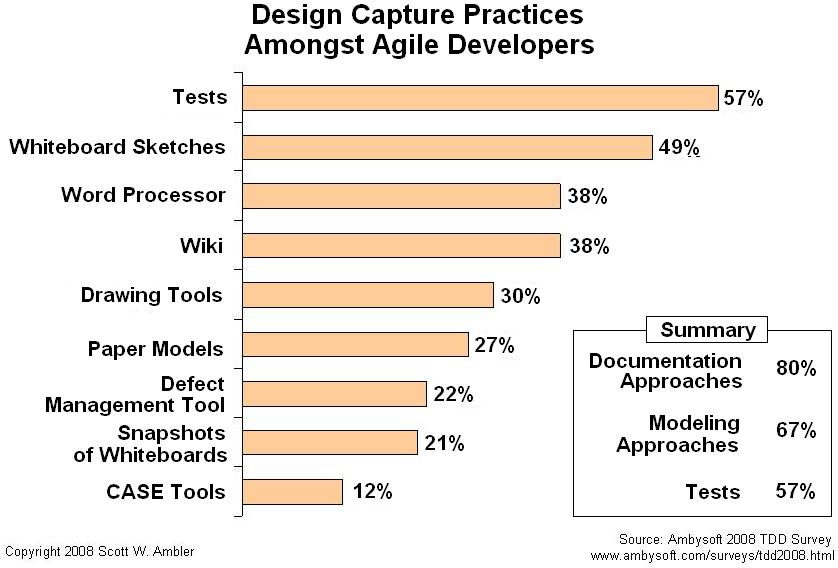
\includegraphics[scale=.4]{tddDesignPractices}
	\caption{Maneiras de captura de design entre desenvolvedores ágeis}   
	\label{fig:wambler-tdd-2008}
\end{figure}			

Entretanto, apesar da quantidade de programadores que adotam a prática, não é
fácil alterar a maneira tradicional de pensar; programadores estão acostumados a
sempre escrever os testes depois de escrever o código. Ao inverter o processo,
programadores são forçados a criar classes que apresentam um bom design.

É realmente difícil entender como TDD influencia no processo de desenvolvimento
de software. Apesar de ter o termo ``teste'' no nome, TDD é uma prática
de design. E, ao contrário do que se espera, boa parte dos experimentos da
academia sobre a prática verificam os efeitos dela sobre a qualidade externa. 

Poucos estudos avaliam TDD do ponto de vista da qualidade interna de código.
Siniaalto e Abrahamsson também compartilham dessa opinião e, além disso, notaram
que os efeitos de TDD podem não ser tão automáticos ou evidentes como o 
esperado \cite{alarming-results}.

Este trabalho visa compreender melhor os efeitos e como a prática de TDD
influencia no design de sistemas orientados a objetos do ponto de vista dos
desenvolvedores que a praticam. 

Esta pesquisa discute três estudos de caso em empresas do mercado brasileiro de
software, que já utilizam TDD normalmente dentro do seu ciclo de
desenvolvimento. Para isso, este trabalho faz uso de métodos qualitativos de
pesquisa, melhor explicados no capítulo \ref{cap:planejamento}.

%% ------------------------------------------------------------------------- %%
\section{Contribuições}

O objetivo desta pesquisa é entender de maneira mais profunda como TDD
influencia no design de sistemas orientados a objetos. Essas informações serão
capturadas baseadas na percepção de programadores que realizam a prática no seu
dia-a-dia de trabalho. Além disso, essa pesquisa se propõe a comparar os
resultados encontrados com os dados existentes na literatura.

A tabela abaixo resume os objetivos da pesquisa:

\begin{itemize}
  \item Entender a influência de TDD no design de sistemas orientados a objetos;

  \item Comparar os resultados encontrados com a literatura existente;
\end{itemize}

Para alcançar esse objetivo, essa pesquisa formulou e tentou responder as
questões listadas abaixo, baseadas nos objetivos:

\begin{itemize}
  \item Como TDD afeta sobre o acoplamento e coesão das classes
  criadas?
  
  \item Como TDD afeta o gerenciamento de dependências em sistemas orientados a
  objetos?

  \item Como TDD afeta a simplicidade das classes criadas?

  \item Como o teste guia o desenvolvedor durante a atividade de
  design?

  \item Qual a relação entre a experiência do desenvolvedor com TDD e
  com sistemas orientados a objetos?
\end{itemize}

%% ------------------------------------------------------------------------- %%
\section{Organização do trabalho}

Este trabalho está dividido da seguinte maneira: 

\begin{itemize}
	\item O Capítulo \ref{cap:tdd} discute o TDD sob o ponto de vista do design.
  
	\item O Capítulo \ref{cap:design} apresenta boa práticas e princípios de design
	que serão investigados durante o processo de entrevistas.

	\item O capítulo \ref{cap:trabalhos-relacionados} mostra trabalhos já
	realizados pela academia sobre os efeitos de TDD.
	
	\item O capítulo \ref{cap:discussao} apresenta os resultados encontrados e
	discute em cima dos mesmos.
	
	\item O capítulo \ref{cap:ameacas} discute as possíveis ameaças dos resultados
	encontrados na pesquisa.
	
	\item O capítulo \ref{cap:conclusoes} resume o trabalho realizado a apresenta
	possibilidades de trabalhos futuros.
\end{itemize}
